\section{Algorithm}
\label{sec:Algorithm}

The algorithm is summarized by this flowchart :
\begin{figure}[!h]
\centering
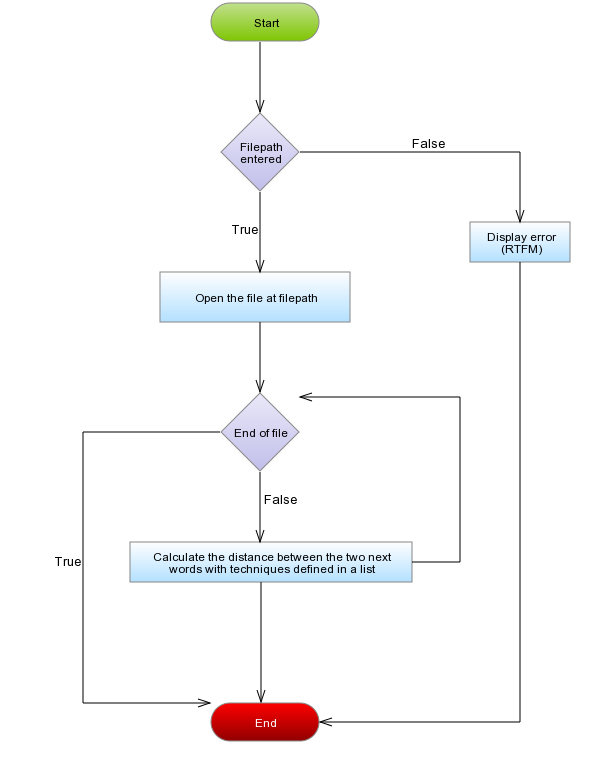
\includegraphics[scale=0.7]{flowchart.png}
\caption{Flowchart of the algorithm}
\label{fig:flowchart}
\end{figure}

Two versions of the algorithm have been implemented : a recursive version and a version using dynamic programming (iterative).

\bigskip
\SetKwProg{Fn}{Function}{}{}
\begin{algorithm}[H]
\Fn{recursiveLevenshteinDistance{(word1 : String, word2 : String)}}{
\If{word1 == word2}{
    \Return{0}
}
lengthWord1 $\leftarrow$ word1.length()\;
lengthWord2 $\leftarrow$ word2.length()\;
\If{lengthWord1 == 0}{
    \Return{lengthWord2}
}
\If{lengthWord2 == 0}{
    \Return{lengthWord1}
}
firstLetterWord1 $\leftarrow$ lengthWord1\;
firstLetterWord2 $\leftarrow$ lengthWord2\;
subWord2 $\leftarrow$ word2.substring(1)\;
subWord2 $\leftarrow$ word2.substring(1)\;
\If{firstLetterWord1 == firstLetterWord2}{
    \Return{recursiveLevenshteinDistance(subWord1, subWord2)}
}
\Else{
    \Return{1 + min(recursiveLevenshteinDistance(subWord1, word2), recursiveLevenshteinDistance(word1, subWord2), recursiveLevenshteinDistance(subWord1, subWord2)}
}
}
\caption{The recursive version of the Levenshtein distance computing algorithm}
\end{algorithm}

\bigskip

\begin{algorithm}[H]
\Fn{dynamicLevenshteinDistance{(word1 : String, word2 : String)}}{
\If{word1 == word2}{
    \Return{0}
}
lengthWord1 $\leftarrow$ word1.length()\;
lengthWord2 $\leftarrow$ word2.length()\;
table $\leftarrow$ int[lengthWord1 + 1, lengthWord2 + 1]\;
\If{lengthWord1 == 0}{\Return{lengthWord2}}
\If{lengthWord2 == 0}{\Return{lengthWord1}}
\For{i $\leftarrow$ 0 to lengthWord1}{
    \For{j $\leftarrow$ 0 to lengthWord2}{
        \If{i == 0}{table[i][j] = j}
        \ElseIf{j == 0}{table[i][j] = i}
        \ElseIf{word1[i - 1] == word2[j - 1]}{table[i][j] = table[i - 1][j - 1]}
        \Else{table[i][j] = 1 + min(table[i - 1][j],  table[i][j - 1], table[i - 1][j - 1]}
    }
}
\Return{table[lengthWord1][lengthWord2]}
}


\caption{The dynamic version of the Levenshtein distance computing algorithm}
\end{algorithm}